% ==========================================================================
\section{Operating System (OS)}
% ==========================================================================
dzOS (or DZOS) is a single-user single-task ROM-based operating system (OS)
for the 8-bit homebrew computer dastaZ80. It is heavily influenced by ideas
and paradigms coming from Digital Research, Inc. CP/M, so some concepts may
sound familiar to those who had used this operating system.

The user communicates with the OS via a keyboard and a screen connected
directly to the computer.

The main job of dzOS is to allow the user to run programs, one at a time and
communicate with the different peripherals (or devices, as referred in this
manual). The user types in a command and the operating system checks what to
do with the command received, to execute a set of instructions.

Other tasks of dzOS are: handling disk files via its file system (DZFS),
getting user input from the keyboard, writing messages on the screen and
receiving/sending data through the serial port.

dzOS consists of three parts:
\begin{itemize}
    \item The \textbf{BIOS}, that provides functions for controlling the
    hardware.
    \item The \textbf{Kernel}, which provides general functions for
    everything that is not hardware dependent.
    \item The Command-Line Interface (\textbf{CLI}), that provides commands
    for the user to talk to the Kernel and the BIOS.
\end{itemize}

The Kernel and the CLI are hardware independent and will work on other Z80
based computers. Therefore, by adapting the BIOS code, dzOS can easily be
ported to other Z80 systems.

    % ==========================================================================
    \subsection{dastaZ80 File System (DZFS)}
    % ==========================================================================
    A file system manages access to the data stored in a storage medium, a
    SD card in the case of dastaZ80, and allows the OS to load and save data in
    the SD card. From now on, referred as \textbf{DISK}.

    DZFS is my first time designing a file system and for this reason I kept it
    very simple.

    It uses Logical Block Addressing (LBA) for accessing the data on the
    \textbf{DISK}, and an allocation table system based in blocks of sectors.
    The allocation table is called Block Allocation Table (BAT).

    Without entering into much details, bytes in the \textbf{DISK} are organised
    as Sectors, and Sectors are grouped into Blocks. Each Sector is 512 bytes
    long and each Block holds 64 Sectors. Therefore, a Block is 32,768 bytes
    long (64 * 512).

    As the free RAM of dastaZ80 is about 48 KB, it makes no sense to have files
    bigger than that, as it would not fit into \textbf{MEMORY}. Therefore, I
    have decided that each Block can store only a single file.

        % ==========================================================================
        \subsubsection{DZFS limitations}
        % ==========================================================================
        The current version of the DZFS implementation (DZFSV1) have the following
        limitations:

        \begin{itemize}
            \item No support for directories. All files are presented at the same
            level.
            \item Filenames:
            \begin{itemize}
                \item Are case sensitive.
                \item Can be maximum 14 characters long.
                \item Can only contain alphabetical (A to Z) and numerical (0 to 9)
                letters.
                \item Cannot start with a number.
                \item No support for extensions. But there is a separate field for
                File Type.
            \end{itemize}
            \item Maximum size for a file is 32,768 bytes.
        \end{itemize}
        
    % ==========================================================================
    \subsection{The Command Prompt}
    % ==========================================================================
    When you switch ON the computer, you will hear a low tone (beep).

    The \textbf{Low Resolution Display} will display a welcome text and the 
    \textbf{High Resolution Display} will show some information:

    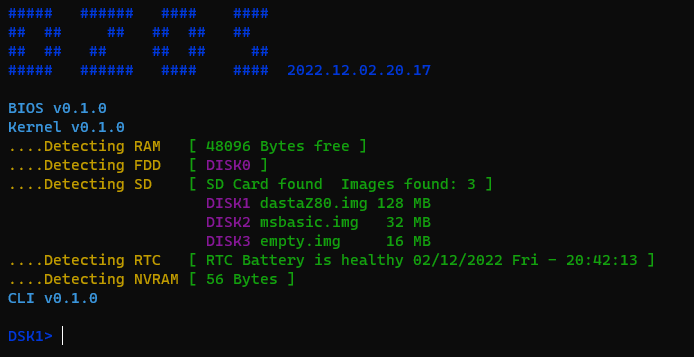
\includegraphics[scale=0.6]{images/dzOS.png}

    This information tells you about the release version of DZOS (2022.07.19.13
    in the screenshot). The BIOS, Kernel and CLI versions, and the detection of
    the different devices used by the computer. It also tells about whichs 
    \textbf{DISK}s are available.

    After that information,you will see the \textit{command prompt}. It starts
    with the letters \textit{DSK} (short for DISK) and a number, followed by the
    symbol $>$

    The number indicates which \textbf{DISK} is currently used for \textbf{DISK}
    operations.

    In other words, if you see \textit{DSK0}, it means that the Floppy Disk Drive
    (\textbf{FDD}) is selected. Entering commands like \textit{cat},
    \textit{diskinfo}, \textit{load}, etc., will instruct the computer to do it
    on the \textbf{FDD}.